\documentclass[10pt,a4paper]{article}
\usepackage[T1]{fontenc}
\usepackage[utf8]{inputenc}
\usepackage{lmodern}
\usepackage[margin=24mm]{geometry}
\usepackage{amsmath,amssymb,amsthm,mathtools}
\usepackage{booktabs,array,graphicx,microtype}
\usepackage[hidelinks]{hyperref}
\hypersetup{pdftitle={Optimizing a Restricted Driving Policy Across a Reduced-Speed Zone},pdfsubject={Empirical fuel modeling and restricted optimal control}}
\usepackage{enumitem}
\usepackage{placeins}
\allowdisplaybreaks
\setlength{\emergencystretch}{2em}
\setlist{nosep,leftmargin=*}
\newcommand{\dd}{\,\mathrm{d}}
\newcommand{\argmin}{\operatorname*{arg\,min}}
\newcommand{\out}{\mathrm{out}}
\newcommand{\inn}{\mathrm{in}}
\newcommand{\cruise}{\mathrm{cr}}
\newcommand{\CZK}{\mathrm{CZK}}
\newtheorem{proposition}{Proposition}
\title{Optimizing a Restricted Driving Policy Across a Reduced-Speed Zone\\[3pt]
\large An empirical fuel model for a \v{S}koda Octavia III Combi 2.0 TDI}
\author{}
\date{Revised 25 September 2026}

\begin{document}
\maketitle
\begin{abstract}
We study a simplified longitudinal driving problem in which travel time, fuel consumption, and expected speeding fines contribute to a monetary objective. Owner-measured steady-speed fuel consumption is fitted directly, without inferring vehicle mass or engine power from fuel use. Published specifications for the facelifted \v{S}koda Octavia III Combi 2.0 TDI provide context for a separate, explicitly approximate dynamics model. A speed-dependent fuel coefficient preserves affine dependence on throttle and exactly reproduces the measured cruise points. Smooth normal Pontryagin extremals admit maximum-propulsion, coasting, full-braking, and singular cruise arcs, but these necessary conditions do not establish a particular global sequence. We therefore optimize an explicitly restricted five-stage family, parameterized by the speeds at the zone boundaries. The resulting problem uses one-dimensional quadratures and a two-variable search, with all alternatives evaluated over the same route. A numerical example compares coasting, full braking, and unchanged-speed travel. Its transition distances depend on assumed mechanical parameters, whereas its cruise-cost calculation is grounded directly in the fuel measurements.
\end{abstract}

\section{Scope and vehicle information}
The objective is a transparent, tractable model of the trade-off between travel time, fuel, and a stylized enforcement penalty. The road is level, traffic-free, and without wind. Gear selection, engine-speed dynamics, transient efficiency, and thermal states are not modeled. The speed limits enter as penalty thresholds, not hard constraints. The computed policy is consequently a monetary optimum for the stated model and admissible family, not a claim about a complete real-world driving objective.

The vehicle is identified as a facelifted \v{S}koda Octavia III Combi 2.0 TDI rated at 110 kW. The 2017 manufacturer data for front-wheel-drive versions are summarized in Table~\ref{tab:factory} \cite{skoda}. The precise model year, transmission, equipment, and loaded mass of the measured car have not been established. The table does not identify a unique vehicle configuration.

\begin{table}[htbp]
\centering
\caption{Manufacturer specifications for the 2017 front-wheel-drive Combi 2.0 TDI, 110 kW \cite{skoda}. Mass includes a 75 kg driver and applies to the basic version. The consumption figures are homologation-cycle results, not constant-speed measurements.}
\label{tab:factory}
\begin{tabular}{@{}lcc@{}}
\toprule
Quantity & Six-speed manual & Six-speed DSG\\
\midrule
Fuel; displacement & \multicolumn{2}{c}{Diesel; 1968 cm$^3$}\\
Maximum engine power & \multicolumn{2}{c}{110 kW at 3500--4000 rpm}\\
Maximum engine torque & \multicolumn{2}{c}{340 Nm at 1750--3000 rpm}\\
Aerodynamic coefficient $C_D$ & \multicolumn{2}{c}{0.302}\\
Kerb mass including driver (kg) & 1354 & 1374\\
Maximum speed (km/h) & 216 & 213\\
Acceleration 0--100 km/h (s) & 8.5 & 8.6\\
Urban consumption (L/100 km) & 5.1 & 5.2\\
Extra-urban consumption (L/100 km) & 3.8 & 4.1\\
Combined consumption (L/100 km) & 4.3 & 4.5\\
\bottomrule
\end{tabular}
\end{table}

The rated engine power is distinct from power delivered at the wheels. Neither rated power nor a test-cycle fuel-consumption figure determines the power needed for steady travel at a particular road speed. No manufacturer constant-speed consumption curve at the three measured speeds was located in the cited material. The owner's measurements therefore remain the calibration targets; the test-cycle values are contextual comparisons only.

\section{Empirical steady-speed fuel consumption}
\label{sec:fuel}
Let $v$ denote the numerical speed in m/s and $V=3.6v$ its value in km/h. Let $Q(v)$ be the moving vehicle's steady fuel rate in L/h. The reported fuel-consumption points are
\begin{equation}
\begin{array}{c|ccc}
V\ (\mathrm{km/h}) & 9 & 80 & 130\\ \hline
\mathrm{FC}_{100}\ (\mathrm{L/100\,km}) & 10.0 & 5.0 & 6.5
\end{array}
\label{eq:measurements}
\end{equation}
and the reported idling baseline is $Q_0=0.6$ L/h. The associated moving fuel rates are 0.9, 4.0, and 8.45 L/h. We use the simple interpolation
\begin{equation}
Q(v)=Q_0+c_1v+c_2v^2+c_3v^3,
\qquad
\mathrm{FC}_{100}(V)=\frac{100}{V}Q(V/3.6).
\label{eq:Qfit}
\end{equation}
Solving the three linear equations obtained from \eqref{eq:measurements} gives
\begin{align}
c_1&=1.20713517724\times10^{-1}\ \frac{\mathrm{L/h}}{\mathrm{m/s}},\notag\\
c_2&=-5.05754823921\times10^{-4}\ \frac{\mathrm{L/h}}{(\mathrm{m/s})^2},\notag\\
c_3&=8.81390936848\times10^{-5}\ \frac{\mathrm{L/h}}{(\mathrm{m/s})^3}.
\label{eq:fitcoeff}
\end{align}
This fit passes through the three moving points and the idling baseline. Its polynomial coefficients are empirical fuel coefficients, not separately identified aerodynamic or rolling-resistance coefficients. The small negative $c_2$ is therefore not a negative physical resistance. On the moving interval $9\le V\le160$ km/h, $Q(v)>Q_0$ and $Q''(v)>0$.

Figure~\ref{fig:fuel} shows the fitted consumption. The $\pm0.5$ L/100 km bars are retained as an illustrative tolerance from the original modeling assumptions; they are not a statistically established measurement uncertainty. Exact interpolation is not independent validation, and the portion above 130 km/h is extrapolation. Road slope, wind, engine temperature, gear, and accessory use should be documented if more measurements become available. The low-speed point helps shape the empirical curve but does not validate a launch or low-speed acceleration model.

\begin{figure}[htbp]
\centering
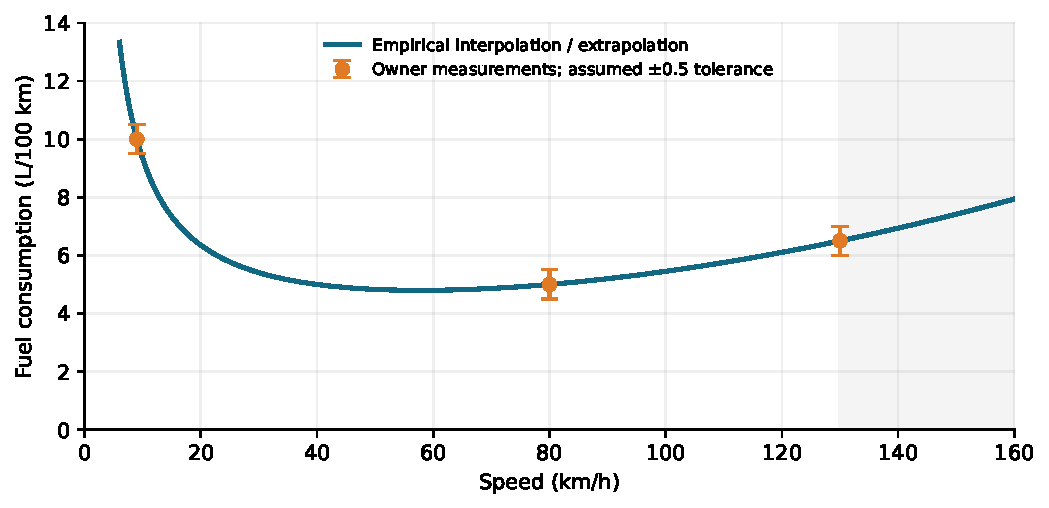
\includegraphics[width=.94\linewidth]{figures/fuel_curve.pdf}
\caption{Steady-speed fuel consumption fitted independently of the mechanical model. The shaded region above 130 km/h is extrapolation. The divergence of consumption per distance as $V\to0$ reflects the positive idling rate; the optimization below stays at positive driving speeds.}
\label{fig:fuel}
\end{figure}

\section{Dynamics and an affine fuel model}
\label{sec:model}
\subsection{Mechanical dynamics and units}
All time-domain equations use seconds, position uses metres, and speed uses m/s. Throttle $u\in[0,1]$ denotes a normalized propulsive command; braking command $b\in[0,1]$ adds a deceleration of $ab$. Write
\begin{align}
\dot x&=v, & \dot v&=h(v)u-R(v)-ab,\label{eq:dynamics}\\
h(v)&=\frac{A}{v+v_0}, & A&=\frac{P_w}{m},\label{eq:h}\\
R(v)&=r_0+r_1v+Bv^2, & B&=\frac{\rho C_D S}{2m}.\label{eq:R}
\end{align}
Here $P_w$ is a wheel-power parameter, $m$ is the assumed moving mass, $S$ is frontal area, and $\rho$ is air density. Thus $A$ has units m$^2$/s$^3$, $B$ has units m$^{-1}$, $r_0$ has units m/s$^2$, and $r_1$ has units s$^{-1}$. A constant-plus-linear-plus-quadratic road load is a standard empirical form \cite{roadload}. For the example we take $r_0=C_{rr}g$ and $r_1=0$.

The regularization $v_0>0$ makes \eqref{eq:h} finite, but the actual propulsive power is
\begin{equation}
P_{\mathrm{traction}}=mh(v)uv=P_wu\frac{v}{v+v_0},
\end{equation}
not exactly $P_wu$. This is a local approximation to power-limited operation, not a torque-and-gear model. We use it for the example on $60\le V\le160$ km/h, not for launching from rest. This interval is a modeling restriction, not a legal speed limit. In general, use a prescribed positive interval $[v_-,v_+]$ on which the approximation is acceptable and $R(v)>0$.

At constant speed without braking,
\begin{equation}
u_{\cruise}(v)=\frac{R(v)}{h(v)}.
\label{eq:ucr}
\end{equation}
Cruising is feasible when $u_{\cruise}(v)\le1$. Transition arcs also require sufficient positive net acceleration wherever acceleration is prescribed.

\subsection{Separating measured fuel use from assumed mechanics}
Define the empirical cruise rate and idle rate in L/s by
\begin{equation}
q_{\cruise}(v)=\frac{Q(v)}{3600},\qquad q_i=\frac{Q_0}{3600}.
\end{equation}
We retain affine dependence on throttle, but allow its slope to depend on speed:
\begin{equation}
\boxed{\dot f=q_i+\Gamma(v)u,
\qquad
\Gamma(v)=\bigl(q_{\cruise}(v)-q_i\bigr)\frac{h(v)}{R(v)}.}
\label{eq:fuelmodel}
\end{equation}
Consequently,
\begin{equation}
q_i+\Gamma(v)u_{\cruise}(v)=q_{\cruise}(v),
\end{equation}
so every measured cruise point is reproduced exactly, independently of the chosen mechanical parameters. On the modeling interval $\Gamma(v)>0$. The original constant-slope fuel law is the special case in which $\Gamma$ happens to be constant.

Equation~\eqref{eq:fuelmodel} is an explicit closure assumption for nonsteady operation. Cruise data alone do not identify fuel use during full acceleration; the chosen affine interpolation supplies that missing information while preserving solvability. In particular, $\dot f=q_i$ during coasting and braking. The coast mode therefore represents engine-running free coasting without modeled engine braking. It does not represent in-gear overrun with fuel cut-off. Adding that mode would require its own deceleration and fuel laws.

\subsection{Illustrative mechanical parameters}
Table~\ref{tab:assumptions} distinguishes published information from assumptions. The mass is a plausible loaded value, not a value inferred from fuel consumption. Neither frontal area, rolling coefficient, nor drivetrain efficiency has been measured on this car.
\begin{table}[htbp]
\centering
\caption{Mechanical inputs for the numerical example. All quantities not explicitly identified as published are scenario assumptions.}
\label{tab:assumptions}
\begin{tabular}{@{}lll@{}}
\toprule
Parameter & Value & Status\\
\midrule
Rated engine power $P_e$ & 110 kW & Manufacturer \cite{skoda}\\
Dimensionless drag coefficient $C_D$ & 0.302 & Manufacturer \cite{skoda}\\
Moving mass $m$ & 1500 kg & Assumed loaded mass\\
Drivetrain factor $\eta_d$ & 0.90 & Assumed\\
Wheel-power parameter $P_w=\eta_dP_e$ & 99 kW & Derived from assumptions\\
Frontal area $S$ & 2.20 m$^2$ & Assumed\\
Air density $\rho$ & 1.225 kg/m$^3$ & Assumed\\
Rolling coefficient $C_{rr}$ & 0.012 & Assumed\\
Gravity $g$; regularizer $v_0$ & 9.81 m/s$^2$; 1 m/s & Fixed approximations\\
Additional full-brake deceleration $a$ & 7 m/s$^2$ & Assumed\\
\bottomrule
\end{tabular}
\end{table}
These give
\begin{equation}
A=66.0\ \mathrm{m^2/s^3},\quad
B=2.712966667\times10^{-4}\ \mathrm{m^{-1}},\quad
r_0=0.11772\ \mathrm{m/s^2},\quad r_1=0.
\label{eq:mechnumbers}
\end{equation}
At 130 km/h the assumed road load requires about 25.54 kW at the wheels. With the measured 8.45 L/h and a representative diesel lower heating value of 35.8 MJ/L \cite{diesel}, this corresponds to approximately 30.4\% overall fuel-to-wheel efficiency. This is a consistency calculation, not an independently measured efficiency. The affine extension predicts about 30.21 L/h at full throttle at that speed, rather than imposing the previous 19 L/h throttle coefficient.

The earlier approximate coast observation, a 130-to-120 km/h reduction in 3--6 s, is not imposed as an exact road-load constraint. It does not specify gear, engine braking, gradient, or wind. For any proposed $R$, the proper comparison is
\begin{equation}
\Delta t_{130\to120}=\int_{120/3.6}^{130/3.6}\frac{\dd v}{R(v)},
\label{eq:coastmeasurement}
\end{equation}
which gives about 6.25 s here, slightly outside that rough interval. Resolving this difference requires a controlled coast-down measurement; it should not be hidden by inferring mass or engine power from fuel use. The transition predictions remain conditional on Table~\ref{tab:assumptions}.

\section{Objective and optimal constant-speed travel}
\label{sec:objective}
\subsection{Time, fuel, and temporal enforcement}
Let $C_t>0$ be the time cost in currency/s and $c_f>0$ the fuel price in currency/L. A reduced-limit zone occupies $x\in[0,L]$. Its regime is $r=\inn$; elsewhere $r=\out$. For each regime, let $v_{\mathrm{lim},r}<v_{\mathrm{hi},r}$ be its two penalty thresholds. Define
\begin{equation}
\phi_r(v)=
\begin{cases}
0,&v\le v_{\mathrm{lim},r},\\
pP_{\mathrm{low}}\lambda_r,&v_{\mathrm{lim},r}<v\le v_{\mathrm{hi},r},\\
pP_{\mathrm{high}}\lambda_r,&v>v_{\mathrm{hi},r},
\end{cases}
\label{eq:fines}
\end{equation}
where $\lambda_r$ is an encounter rate in s$^{-1}$, $p\in[0,1]$ a charge probability, and the $P$'s are nonnegative fine amounts with $P_{\mathrm{high}}>P_{\mathrm{low}}$. This is an expected cumulative penalty under an additive repeated-event model, for example independently chargeable Poisson encounters. A one-fine-per-trip model or enforcement per unit distance would give a different objective. No claim is made that these illustrative amounts reproduce current traffic law.

The running cost is
\begin{equation}
\ell_r(v,u)=C_t+c_f\bigl(q_i+\Gamma(v)u\bigr)+\phi_r(v).
\label{eq:running}
\end{equation}
For fixed $U,W>0$, the general route problem minimizes
\begin{equation}
J=\int_0^T\ell_{r(x(t))}(v(t),u(t))\dd t
\label{eq:objective}
\end{equation}
over measurable controls satisfying \eqref{eq:dynamics}, $u,b\in[0,1]$, and $v\in[v_-,v_+]$, subject to
\begin{equation}
x(0)=-U,\quad x(T)=L+W,\quad v(0)=v(T)=v_{\out}.
\end{equation}
Terminal time $T$ is free and there is no terminal cost. The reference speed $v_{\out}$ is selected below, then held fixed when comparing trajectories.

\subsection{Cruise cost and candidate speeds}
For feasible constant-speed travel,
\begin{equation}
g_r(v)=\frac{C_t+c_fq_{\cruise}(v)+\phi_r(v)}{v},\qquad
v_r\in\argmin_{\substack{v\in[v_-,v_+]\\R(v)\le h(v)}}g_r(v).
\label{eq:g}
\end{equation}
The empirical fuel data enter this calculation directly. The mechanical model only determines which cruising speeds are feasible. Within a band where $\phi_r$ is constant, an interior stationary point satisfies
\begin{equation}
c_f\bigl[vq'_{\cruise}(v)-q_{\cruise}(v)\bigr]=C_t+\phi_r.
\label{eq:cruisestationary}
\end{equation}
For \eqref{eq:Qfit}, this becomes the cubic equation
\begin{equation}
2c_3v^3+c_2v^2-Q_0=\frac{3600}{c_f}(C_t+\phi_r).
\label{eq:cubic}
\end{equation}
One compares admissible roots with all feasible domain endpoints, fine thresholds, and any sustainable-speed endpoint $h(v)=R(v)$. Thresholds are evaluated using the convention in \eqref{eq:fines}; their upward jumps can create minima without satisfying \eqref{eq:cruisestationary}. A sustainable-speed endpoint may be feasible for cruise but unreachable in finite time along a maximum-acceleration arc.

In the restricted construction below assume $v_{\inn}<v_{\out}$ and strictly positive net acceleration between them. If the selected speeds coincide, no transition is needed. If their order reverses, the assumed deceleration--acceleration sequence is inapplicable; a lower posted limit alone does not guarantee this ordering when enforcement intensities differ.

\section{What the maximum principle establishes}
\label{sec:pmp}
\subsection{Smooth normal extremals}
The following calculations apply to normal extremals on intervals away from fine thresholds, spatial regime boundaries, and active speed-domain constraints. We use the Hamiltonian minimization convention \cite{liberzon}:
\begin{equation}
H_r=C_t+c_fq_i+\phi_r(v)+c_f\Gamma(v)u
       +\psi_xv+\psi_v\bigl(h(v)u-R(v)-ab\bigr).
\label{eq:H}
\end{equation}
The cost multiplier has been normalized to one; abnormal extremals are not excluded by this local calculation. The costate equations on a smooth interval are
\begin{align}
\dot\psi_x&=0,\notag\\
\dot\psi_v&=-\phi'_r(v)-c_f\Gamma'(v)u-\psi_x
             -\psi_v\bigl(h'(v)u-R'(v)\bigr).
\label{eq:costates}
\end{align}
The switching functions are
\begin{equation}
\sigma_u=c_f\Gamma(v)+\psi_vh(v),\qquad \sigma_b=-a\psi_v.
\end{equation}
Thus $u=0$ if $\sigma_u>0$ and $u=1$ if $\sigma_u<0$; $b=0$ if $\psi_v<0$ and $b=1$ if $\psi_v>0$. At a zero, pointwise minimization alone leaves the corresponding control undetermined. A singular arc requires the switching function to vanish on an interval, not just at an isolated switching instant. Since $\Gamma,h>0$, the nonsingular choices are maximum propulsion without braking, coasting, and full braking without propulsion.

\subsection{Singular cruise arcs}
Define
\begin{equation}
K(v)=\frac{c_f\Gamma(v)}{h(v)}
     =\frac{c_f\bigl(q_{\cruise}(v)-q_i\bigr)}{R(v)}>0.
\label{eq:K}
\end{equation}
On a throttle-singular interval, $\psi_v=-K(v)<0$, hence $b=0$. Differentiating this relation and using \eqref{eq:costates}, in a band where $\phi'_r=0$, yields
\begin{equation}
\psi_x=-\bigl[K(v)R(v)\bigr]'=-c_fq'_{\cruise}(v).
\label{eq:singularx}
\end{equation}
Since $\psi_x$ is constant, $q''_{\cruise}(v)\dot v=0$. The fit in Section~\ref{sec:fuel} has $q''_{\cruise}>0$ throughout the driving interval, so a smooth throttle-singular arc must have constant speed and throttle $u=R/h$. For the autonomous free-terminal-time problem, $H=0$ on a normal extremal \cite{liberzon}. Substituting \eqref{eq:singularx} in \eqref{eq:H} then recovers \eqref{eq:cruisestationary}.

These are necessary consistency conditions. Merely selecting a feasible constant speed and an interior throttle does not automatically produce an extremal or an optimum. A smooth brake-singular interval would have $\psi_v=0$, then $u=0$ and $\psi_x=0$ by \eqref{eq:costates}. Its Hamiltonian would be $C_t+c_fq_i+\phi_r>0$, contradicting $H=0$. Thus such an interval is absent under these smooth normal free-time assumptions.

\subsection{Discontinuities and the restricted-family interpretation}
The discontinuous penalty is not covered everywhere by the smooth calculation. In particular, $\phi'_r(v)=0$ almost everywhere as a function of speed does not justify ignoring a trajectory that remains at a threshold for a positive time. A threshold cruise is handled directly in the finite-dimensional optimization below; we do not assert that it is an ordinary smooth singular arc.

For an isolated transverse crossing of $x=0$ or $x=L$, away from simultaneous speed-threshold events, the usual hybrid corner conditions with no state reset or switching cost give continuity of $H$ and $\psi_v$, while $\psi_x$ may jump \cite{hybrid}. With the same dynamics on both sides,
\begin{equation}
\psi_x^+-\psi_x^-=-\frac{\phi_{r^+}(v)-\phi_{r^-}(v)}{v}.
\end{equation}
The control switching functions remain continuous; a spatial boundary does not itself force a control switch. Speed-threshold crossings and threshold residence require separate nonsmooth treatment if one seeks a theorem for the unrestricted problem.

PMP therefore motivates useful control types but does not establish their number, order, or global optimality. The next section explicitly restricts the trajectory family. It excludes mixed coast--brake deceleration, arbitrary additional switches, and trajectories whose minimum speed is above the chosen inside cruise speed.

\section{Five-stage family and transition quadratures}
\label{sec:family}
Fix feasible reference speeds $v_{\inn}<v_{\out}$ from \eqref{eq:g}. The five stages are: outside cruise at $v_{\out}$; deceleration to $v_{\inn}$; inside cruise at $v_{\inn}$; maximum acceleration back to $v_{\out}$; and outside cruise at $v_{\out}$. Deceleration is either entirely coasting or entirely full braking. Zero-length cruise stages are allowed. We require
\begin{equation}
R_d(v)=R(v)+ab_d>0,\quad b_d\in\{0,1\},\qquad
F(v)=h(v)-R(v)>0
\label{eq:denominators}
\end{equation}
on $[v_{\inn},v_{\out}]$. The total distances are
\begin{equation}
D_d=\int_{v_{\inn}}^{v_{\out}}\frac{v}{R_d(v)}\dd v,
\qquad
D_a=\int_{v_{\inn}}^{v_{\out}}\frac{v}{F(v)}\dd v.
\end{equation}
They follow from $\dd x/\dd v=v/\dot v$.

\subsection{Boundary-speed parametrization}
Require the deceleration arc to touch or cross $x=0$ and the acceleration arc to touch or cross $x=L$. Define
\begin{equation}
v_b=v(x=0),\qquad v_c=v(x=L),\qquad
(v_b,v_c)\in[v_{\inn},v_{\out}]^2.
\end{equation}
These are spatial evaluations, not the initial and terminal speeds at times 0 and $T$. The split distances are
\begin{align}
D_d^{\out}(v_b)&=\int_{v_b}^{v_{\out}}\frac{v}{R_d(v)}\dd v,&
D_d^{\inn}(v_b)&=\int_{v_{\inn}}^{v_b}\frac{v}{R_d(v)}\dd v,\notag\\
D_a^{\inn}(v_c)&=\int_{v_{\inn}}^{v_c}\frac{v}{F(v)}\dd v,&
D_a^{\out}(v_c)&=\int_{v_c}^{v_{\out}}\frac{v}{F(v)}\dd v.
\label{eq:splitdist}
\end{align}
Their sums are $D_d$ and $D_a$, independent of boundary speeds for fixed reference speeds and deceleration mode. The switching positions are
\begin{equation}
x_{12}=-D_d^{\out},\quad x_{23}=D_d^{\inn},\quad
x_{34}=L-D_a^{\inn},\quad x_{45}=L+D_a^{\out}.
\label{eq:switchpositions}
\end{equation}
The inside-cruise length is
\begin{equation}
L_{\cruise}=L-D_d^{\inn}(v_b)-D_a^{\inn}(v_c)\ge0.
\label{eq:feasibility}
\end{equation}
This family includes the four endpoint combinations, but also allows intermediate boundary speeds. It does not include arbitrary translations of a transition entirely away from its associated boundary.

\subsection{Transition costs}
Define deceleration and acceleration cost integrands by
\begin{equation}
L_{d,r}(v)=C_t+c_fq_i+\phi_r(v),\qquad
L_{a,r}(v)=C_t+c_f\bigl(q_i+\Gamma(v)\bigr)+\phi_r(v).
\end{equation}
Then
\begin{align}
J_d^{\out}(v_b)&=\int_{v_b}^{v_{\out}}\frac{L_{d,\out}(v)}{R_d(v)}\dd v,&
J_d^{\inn}(v_b)&=\int_{v_{\inn}}^{v_b}\frac{L_{d,\inn}(v)}{R_d(v)}\dd v,\notag\\
J_a^{\inn}(v_c)&=\int_{v_{\inn}}^{v_c}\frac{L_{a,\inn}(v)}{F(v)}\dd v,&
J_a^{\out}(v_c)&=\int_{v_c}^{v_{\out}}\frac{L_{a,\out}(v)}{F(v)}\dd v.
\label{eq:splitcost}
\end{align}
These are one-dimensional quadratures. Split numerical integration at every fine threshold to avoid integrating blindly across a jump. The additional speed dependence of $\Gamma$ changes the acceleration integrand but does not increase the optimization dimension.

\section{A common route and a finite-dimensional optimization}
\label{sec:optimization}
Let $G_{\out}=g_{\out}(v_{\out})$ and $G_{\inn}=g_{\inn}(v_{\inn})$. Choose the same $U,W$ for every comparison, with
\begin{equation}
U\ge\max_{b_d\in\{0,1\}}D_d,\qquad W\ge D_a.
\end{equation}
The outside cruise distances are $U-D_d^{\out}$ before deceleration and $W-D_a^{\out}$ after acceleration. Therefore
\begin{equation}
\boxed{\begin{aligned}
J_d(v_b,v_c)={}&G_{\out}\bigl[U+W-D_d^{\out}(v_b)-D_a^{\out}(v_c)\bigr]\\
&+G_{\inn}\bigl[L-D_d^{\inn}(v_b)-D_a^{\inn}(v_c)\bigr]\\
&+J_d^{\out}(v_b)+J_d^{\inn}(v_b)
 +J_a^{\inn}(v_c)+J_a^{\out}(v_c).
\end{aligned}}
\label{eq:totalcost}
\end{equation}
Minimize this expression over \eqref{eq:feasibility} separately for each deceleration mode, then compare the two minima. Evaluating each mode on its own window $[-D_d,L+D_a]$ is invalid for the cross-mode comparison, since full braking traverses a shorter route. If such mode-specific costs have already been computed, add
\begin{equation}
G_{\out}\bigl[(U-D_d)+(W-D_a)\bigr]
\end{equation}
to obtain costs on the common route.

\subsection{Interior candidates and discontinuity candidates}
For fixed mode, \eqref{eq:totalcost} separates into a constant, a function of $v_b$, and a function of $v_c$. Define
\begin{equation}
\Delta\phi(v)=\phi_{\inn}(v)-\phi_{\out}(v),\qquad
N(v)=(G_{\out}-G_{\inn})v+\Delta\phi(v).
\end{equation}
Away from thresholds,
\begin{equation}
\frac{\partial J_d}{\partial v_b}=\frac{N(v_b)}{R_d(v_b)},\qquad
\frac{\partial J_d}{\partial v_c}=\frac{N(v_c)}{F(v_c)}.
\label{eq:partials}
\end{equation}
All fuel and time terms on a given transition cancel in this derivative because moving the regime boundary changes only its fine rate and the displaced cruise distances. Thus the boundary-speed equations retain the same simple form even with speed-dependent throttle fuel use.

In each common fine band, a stationary candidate is
\begin{equation}
v^*=-\frac{\Delta\phi}{G_{\out}-G_{\inn}},
\end{equation}
provided the denominator is nonzero and the root lies in the band and in $[v_{\inn},v_{\out}]$. Add the interval endpoints and every fine threshold in that interval. The transition-cost integrals themselves are continuous as functions of their limits, but have derivative changes at the thresholds.

If $G_{\out}=G_{\inn}$, derivatives have the sign of $\Delta\phi$ within each band; if $\Delta\phi=0$ as well, that band's contribution is flat. Flat candidate intervals must be retained, rather than discarded by division by zero. If independent global minimizers of the two separated terms are feasible, their combination is globally optimal within the fixed-mode family. Otherwise evaluate all feasible candidate combinations and the active constraint below. First-order roots alone do not guarantee minima.

\subsection{Active inside-length constraint}
On the active boundary,
\begin{equation}
D_d^{\inn}(v_b)+D_a^{\inn}(v_c)=L.
\end{equation}
For every $v_b$ for which $L-D_d^{\inn}(v_b)\in[0,D_a]$, determine the unique $v_c(v_b)$ by inversion of the strictly increasing function $D_a^{\inn}$. The problem becomes a one-dimensional minimization of $J_d(v_b,v_c(v_b))$. Split this search at both entry and exit fine-threshold events and include its endpoints. On a smooth portion,
\begin{equation}
\frac{\dd}{\dd v_b}J_d(v_b,v_c(v_b))
=\frac{\Delta\phi(v_b)-(v_b/v_c)\Delta\phi(v_c)}{R_d(v_b)}.
\label{eq:activeDerivative}
\end{equation}
This supplies additional stationary candidates or identifies a flat portion. Comparing all these candidates gives the global minimum of the restricted two-variable problem, including its boundary. The feasible set is compact and the objective is continuous under the stated positive-denominator assumptions, so a restricted minimum exists.

An active constraint means only that the prescribed inside cruise has zero length. It does not prove that an unrestricted short-zone optimum reaches $v_{\inn}$. A useful extension is to optimize a turning speed $w\in[v_{\inn},v_{\out}]$, replace the lower integration limits by $w$, and use $g_{\inn}(w)$ for any inside plateau. Another is to add a coast--brake switching speed. Both remain finite-dimensional restrictions, without establishing unrestricted global optimality. Constant-speed travel at $v_{\out}$ should also be compared as a separate baseline.

\section{An exact identity for checking costs}
\label{sec:identity}
Let $\Xi'(v)=K(v)$ with $K$ from \eqref{eq:K}. Eliminating throttle from \eqref{eq:dynamics} and \eqref{eq:fuelmodel} gives
\begin{equation}
\boxed{
J=\Xi(v(T))-\Xi(v(0))
 +\int_{x(0)}^{x(T)}g_{r(x)}(v(x))\dd x
 +\int_0^T K(v(t))ab(t)\dd t.}
\label{eq:identity}
\end{equation}
Indeed $c_f\Gamma u=K\dot v+KR+Kab$, while $KR=c_f(q_{\cruise}-q_i)$. With equal initial and final speeds, the endpoint term cancels. This identity is an algebraic property of the assumed affine fuel model, not a general law of vehicle energetics. It provides an independent check of time-domain or quadrature-based cost calculations and displays the explicit braking penalty. It does not imply that braking can never be optimal: braking can change the speed profile, fines, travel time, and the available transition distance.

\section{Numerical example}
\label{sec:numerical}
\subsection{Economic inputs and reference speeds}
Use the mechanical inputs in Table~\ref{tab:assumptions}, the fuel interpolation \eqref{eq:Qfit}, and
\begin{align}
L&=1000\ \mathrm{m},&U&=2000\ \mathrm{m},&W&=2000\ \mathrm{m},\notag\\
C_t&=300/3600\ \CZK/\mathrm{s},&c_f&=32\ \CZK/\mathrm{L},&p&=1,\notag\\
\lambda_{\out}&=\lambda_{\inn}=0.026/3600\ \mathrm{s^{-1}},\notag\\
P_{\mathrm{low}}&=2500\ \CZK,&P_{\mathrm{high}}&=15000\ \CZK.
\end{align}
The outside thresholds are 130 and 160 km/h, and the inside thresholds are 80 and 110 km/h. The two nonzero fine rates are consequently 65/3600 and 390/3600 CZK/s. All variants cover the same 5 km route from $x=-2000$ to $x=3000$ m.

Minimizing \eqref{eq:g} on the assumed 60--160 km/h driving interval gives
\begin{equation}
v_{\out}=130\ \mathrm{km/h},\qquad v_{\inn}=110\ \mathrm{km/h},
\end{equation}
with
\begin{equation}
1000G_{\out}=4.38769\ \CZK/\mathrm{km},\qquad
1000G_{\inn}=5.15984\ \CZK/\mathrm{km}.
\end{equation}
At 80 km/h the inside cruise cost is 5.35000 CZK/km. The model therefore chooses 110 km/h in the nominal 80 km/h zone. At exactly 110 km/h the lower fine applies; immediately above it the higher fine applies. This threshold convention is consequential. Both selected cruise speeds are threshold minima rather than roots of the smooth cruise-stationarity equation.

For $110<V<130$ km/h, $\Delta\phi=390/3600$ CZK/s and $N(v)>0$. Hence both partial derivatives in \eqref{eq:partials} are positive throughout the open interval. For either deceleration mode, the restricted minimum is
\begin{equation}
v_b^*=v_c^*=110\ \mathrm{km/h}.
\end{equation}
Deceleration finishes at the zone entrance and acceleration starts at its exit. The inside-length constraint is inactive. This proves the boundary-speed minimum for this example, without asserting that the restricted sequence is the global solution of \eqref{eq:objective}.

\subsection{Costs, distances, and interpretation}
Table~\ref{tab:results} gives the common-route comparison. The unchanged-speed baseline remains at 130 km/h throughout, including the zone, and is outside the five-stage family with a prescribed lower cruise speed.
\begin{table}[htbp]
\centering
\caption{Computed results on the same 5 km route. Values are conditional on the assumed mechanics and transient fuel law. Expected fines are monetary expectations, not guaranteed payments.}
\label{tab:results}
\begin{tabular}{@{}lrrr@{}}
\toprule
Quantity & Coasting family & Full-braking family & Constant 130 km/h\\
\midrule
Deceleration distance (m) & 441.71 & 24.95 & ---\\
Acceleration distance (m) & 124.15 & 124.15 & ---\\
Travel time (s) & 144.83 & 143.83 & 138.46\\
Fuel (L) & 0.31537 & 0.34037 & 0.32500\\
Expected fines (CZK) & 0.59091 & 0.59091 & 3.00000\\
Total cost (CZK) & \textbf{22.75225} & 23.46836 & 24.93846\\
\bottomrule
\end{tabular}
\end{table}

Relative to full braking, the coasting profile takes about 1.01 s longer and consumes about 0.02500 L less fuel. The time penalty is about 0.08382 CZK, the fuel saving about 0.79993 CZK, and the net saving about 0.71611 CZK. Relative to unchanged-speed travel, it takes about 6.37 s longer and lowers the modeled total cost by about 2.18621 CZK.

The coasting switching positions are approximately
\begin{equation}
(x_{12},x_{23},x_{34},x_{45})=(-441.71,0,1000,1124.15)\ \mathrm{m}.
\end{equation}
The profile is shown in Figure~\ref{fig:profile}. Its instantaneous cost per distance is $1000\ell_r(v,u)/v$ in CZK/km. This differs from the cruise density $1000g_r(v)$ on acceleration and deceleration arcs. Jumps at control changes are expected in the affine model; isolated endpoint values do not affect the integrals.

\begin{figure}[!t]
\centering
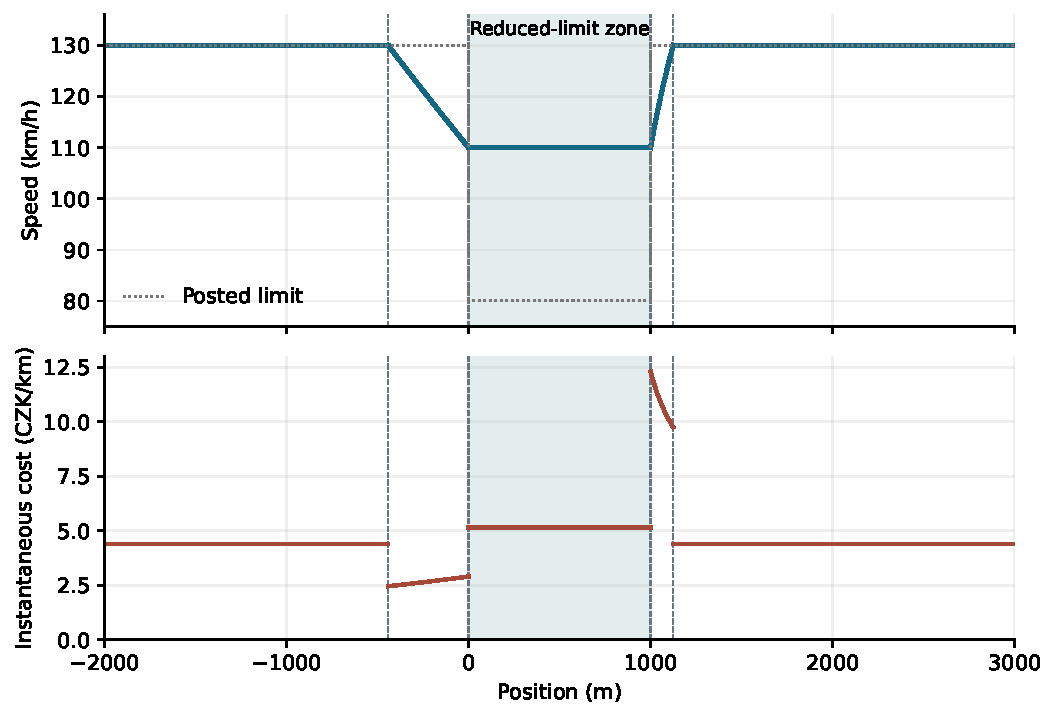
\includegraphics[width=.96\linewidth]{figures/speed_profile.pdf}
\caption{Minimum-cost coasting profile within the prescribed boundary-speed family, with instantaneous monetary cost per distance shown separately. The shaded zone has an 80 km/h posted limit. The model chooses a 110 km/h plateau because of its specified time valuation and expected-fine schedule. Dashed vertical lines mark the four control changes.}
\label{fig:profile}
\end{figure}

\section{Limitations and measurements that would improve the model}
The fuel interpolation, the assumed road load, and the assumed transient fuel law play different roles. Changing the road load or wheel-power parameter while retaining \eqref{eq:fuelmodel} preserves the measured cruise curve and its unconstrained economic minimizers, provided those speeds remain feasible. It changes transition distances, transition fuel use, and the total route cost. Agreement at the three cruise points cannot select among such mechanical models.

The most useful additional data would be a known loaded mass, repeated level-road coast-down times with gear and clutch state recorded, and timed acceleration with simultaneous fuel measurements over the actual transition-speed range. Fuel cut-off and engine braking should be introduced together as a separate control mode if they are important in the measured vehicle. An energy-efficiency map or full transmission model is not needed merely to optimize the present restricted family.

The example's numerical precision serves reproducibility, not a claim of equally precise prediction. Uncertainty in fuel measurements, road load, enforcement intensity, and the value of time can change the selected policy. The sharp fine thresholds can also favor exact-threshold speeds; a smoothed or uncertain threshold would be a different modeling choice.

\section{Conclusion}
Direct interpolation of measured fuel consumption avoids an unsupported conversion from fuel use to engine power or vehicle mass. A speed-dependent coefficient in an otherwise affine throttle law preserves the mathematical structure needed for simple cruise optimization, local PMP calculations, and transition quadratures. Smooth singular-cruise conditions can be derived explicitly, while fine-threshold cruises and the choice of a five-stage sequence are treated separately. Optimizing two boundary speeds gives an exact minimum within the prescribed family, and a fixed spatial window permits meaningful comparison between coasting, braking, and baseline travel. Under the illustrative inputs, coasting to 110 km/h before the zone and accelerating after it has the lowest cost among the compared alternatives; its transition distances remain conditional on unmeasured mechanical and transient-fuel assumptions.

\appendix
\section{Reproducibility}
The accompanying \texttt{reproduce.py} requires Python 3, NumPy, SciPy, and Matplotlib. It solves the fuel interpolation, enumerates cruise candidates, evaluates the transition quadratures, checks both the time--fuel--fine decomposition and the exact cost identity, and generates the figures and \texttt{results.json}. Run it from any working directory, then compile this file with \texttt{pdflatex article.tex} twice from the source directory. Pre-generated PDF figures are supplied, so Python is not needed simply to compile the article. The original supplied illustrations were inspected as references; both figures here are regenerated from the revised model.

\begin{thebibliography}{9}
\bibitem{skoda}
\v{S}KODA AUTO, \emph{87th Geneva International Motor Show: Press Kit}, 7 March 2017, PDF pp.~59--61, ``\v{S}KODA OCTAVIA COMBI: Diesel engines.''
\url{https://cdn.skoda-storyboard.com/2017/03/170307-Geneva-2017-Press-Kit.pdf}.
\bibitem{roadload}
U.S. Environmental Protection Agency, \emph{Population and Activity of Onroad Vehicles in MOVES5}, Section~15, ``Vehicle Mass and Road Load Coefficients.''
\url{https://nepis.epa.gov/Exe/ZyPURL.cgi?Dockey=P101CUN7.TXT}.
\bibitem{diesel}
U.S. Department of Energy, Alternative Fuels Data Center, \emph{Fuel Properties Comparison}, low-sulfur diesel lower heating value (approximately 35.8 MJ/L).
\url{https://afdc.energy.gov/fuels/properties}.
\bibitem{liberzon}
D.~Liberzon, \emph{Calculus of Variations and Optimal Control Theory: A Concise Introduction}. Princeton University Press, 2012. Sections~4.1.1 and 4.4.3; author's online version:
\url{https://liberzon.csl.illinois.edu/teaching/cvoc/node63.html} and
\url{https://liberzon.csl.illinois.edu/teaching/cvoc/node87.html}.
\bibitem{hybrid}
A.~Pakniyat and P.~E.~Caines, ``On the Hybrid Minimum Principle: The Hamiltonian and Adjoint Boundary Conditions,'' \emph{IEEE Transactions on Automatic Control}.
\url{https://ieeexplore.ieee.org/document/9086153/}.
\end{thebibliography}
\end{document}
